\chapter{Unconventional instruments}\label{chap:unconventional}

`Does it have to look like an instrument?' one of my students asked. It was the first time I was teaching a course in sound programming, and I had given them the assignment to design and build an electro-acoustic instrument. Most of the students had plans for making software-based designs, possibly hooking up a MIDI controller for the interaction. The question sparked off an interesting discussion about the visual appearance of instruments. What does an instrument really look like? Is it possible to design an instrument that does not look like an instrument? These questions have been with me ever since. Over the years, I have created various instruments. Mainly electro-acoustic, but also some acoustic. In recent years, I have become more interested in hybrid devices that bridge between acoustic and electro-acoustic instruments. In this chapter, I will present some of my unconventional instruments and controllers. These are designed to be different. Similar to the impossible instruments mentioned in Chapter~\ref{sec:imaginary}, unconventional instruments are not only sound-makers. Equally important is how they challenge our thinking about what an instrument can be.


\section{An action--sound design philosophy}

There is no universal recipe for the design of new instruments; there are just too many variables involved. It is not difficult to make an instrument. Anyone can construct an instrument with whatever materials they have around. Music technology educators have long experience teaching students how to build simple acoustic and electro-acoustic instruments. We probably also have many different strategies for how to make students succeed in developing new instruments.

In many ways, this book summarizes my instrument design philosophy. Some may find it strange that I spend so much time dealing with non-technological topics. When I began teaching music technology courses, my approach was very technology-focused. I taught the students about the knuts and bolts of signal processing, sensor interfaces, and programming. I ensured that they mastered sound synthesis before we moved on to control the sound engines. It was a structured approach to electro-acoustic instrument development, but it was not very inspiring. It was also an utterly disembodied approach.

Over time, I gradually developed what I have called an action--sound design philosophy \citep{jensenius_action-sound_2013}. This is based on the embodied cognition theory we looked at in Chapter~\ref{chapter:music-cognition}. In particular, I have been fascinated by how the human body interacts with the world through objects. \citet{papanek_design_1985} has written about the need to design for the `real world.' One approach to doing that is by embracing the affordance theory of \citet{gibson_theory_1977} and its application to design theory by \citet{norman_design_1990, norman_design_2013}. In his books on the design of everyday things, Norman focuses on creating intuitive objects. They should feel `natural' to the user, whether it is constructing a door handle, a teapot, or computer software.
Later on, he has also called for the need for more \emph{emotional design} \citep{norman_emotional_2004}, which in many ways overlaps with thoughts on \emph{affective computing} \citep{picard_affective_1997-1}. A red line through all these design approaches is that new technologies need to be embodied and human-focused. When working with computer-based systems, it is easy to end up with technology-oriented solutions. That is because we are developing based on the computer's logic. However, how can we design for humans?

\citet{wang_artful_2018} suggests that we should aim for creating \emph{sublime} designs. One of his strategies to reach such sublimity is by creating `playful' designs. This will make users physically and emotionally engaged. This resonates with how \citet{norman_emotional_2004} suggests that we need to take three levels of human processing into account when creating designs:

\begin{itemize}
\item Visceral: the automatic, prewired layer
\item Behavioral: the brain processes that control everyday behavior
\item Reflective: the contemplative part of the brain
\end{itemize}

A challenge is how to achieve all such design ideas when `anything' is possible, particularly with computer-based instruments. It is like bringing someone into a large workshop and ask them to make `anything.' That may be a more difficult task than giving them a small piece of paper, a stencil, and three colored pencils. Limiting peoples' possibilities fosters creativity.
\citet{magnusson_epistemic_2009} argues that electro-acoustic instruments should be developed based on a \emph{constraint-based design}. Too many possibilities are daunting to a user. Therefore, designing constraints into devices helps trigger action. These constraints may, in turn, spark off novel usage. As \citet{magnusson_ergomimesis_2018} writes, the instruments may `teach, adapt, explain, direct, suggest, entice'.

In his `laws of simplicity,' \citet[89]{maeda_laws_2006} suggested that `[s]implicity is about subtracting the obvious, and adding the meaningful.' However, what does simplicity mean when it comes to musical instrument design? Many acoustic instruments require years of practice to master. Hence, only a few musicians will ever reach a level of virtuosity on their instruments. Still, many people manage to get started with an acoustic instrument quickly. For example, most will produce sound the first time they pick up a guitar. Many also learn to play a few chords and a scale in a relatively short time. However, to move from novice to master is, indeed, a long journey.

\citet{wessel_problems_2001} argued that simple controllers lead to simple interaction. Such devices may feel more like a toy than an instrument, which may discourage continued musical exploration. Instead, the aim should be to create instruments that have a `low entry fee with no ceiling on virtuosity' \citep{wright_problems_2002}. They later regretted that phrase, suggesting instead to focus on designing `high-ceiling toys' \citep{jensenius_unsolved_2017}.

In my thinking, one approach to designing such high-ceiling toys is by increasing the spatiotemporal resolution of the controllers. Adding multidimensional control is another way of increasing the interaction possibilities of an interface. However, as discussed in Chapter~\ref{sec:mpe-instruments}, adding more possibilities may also increase the cognitive load. Then it may help to leverage on the \emph{idiomatic} nature of existing instruments, building on what feels `natural' to play on a particular device. \citet{tahiroglu_contextualising_2018} have argued that:

\begin{quotation}
A gesture vocabulary that is idiomatic to the new musical instrument establishes a set of playing techniques for that instrument, which is, in turn, an essential component of developing a performance practice.
\end{quotation}

Several other researchers have argued for the need to consider idiomaticity more carefully, in both acoustic \citep{aho_tangible_2016, de_souza_music_2017} and electro-acoustic \citep{frisk_improvisation_2008,mcpherson_idiomatic_2020} musicking. However, idiomaticity may come in different forms and is highly dependent on the mappings between action and sound. If the mappings work well, an instrument is typically also experienced as both intuitive and simple to use.

Simplicity can take different forms whether we think about instruments as sound-makers or music-makers. For example, accompaniment keyboards focus on maximizing the musical output while reducing the interaction complexity. Such instruments often target beginners and build on the idiomaticity of the piano keyboard. At the same time, these instruments embody much musical knowledge through built-in sound and music engines. Through the touch of a button, the user can play an accompaniment (primarily chords and rhythms) following the melody played by the user. As such, the musical output is much more complex than what would be achievable with a traditional sound-maker. Nevertheless, the user controls the musical output, but not beyond the musical structures pre-programmed into the instrument.

We have just seen the beginning of such semi-automatic instruments. In the future, I am sure that different types of machine musicianship will be the norm.
Some may find this problematic, but almost twenty years ago \citet[171]{machover_shaping_2004} argued for the benefits of such an active approach to music:

\begin{quote}
	What if we could unlock the expressive mysteries of music first, before learning the technical foundations, if we could help young people---and others---fall in love with the joys of music first, subsequently demanding deeper knowledge once they were `hooked'?
\end{quote}

In the Toy Symphony and other projects at the MIT Media Lab, Machover has explored semi-automatic instruments that allow for active musicking. The users, often children, perform complex music with simple, toy-like controllers. The idea is that the instruments should be immediately easy-to-use yet provide rich musical experiences. The instruments may not allow for developing virtuosity, but they create excitement through musicking. That has also been one of the goals of my instrument designs.


\section{Cheapstick}\label{sec:cheapstick}

My explorations into new instrument design came through software development. Then one typically puts together existing hardware and focuses on programming mappings between controllers and sound engines.
\emph{Cheapstick} was my first attempt at creating a hardware controller \citep{jensenius_building_2006}. Nowadays, there are numerous affordable sensor interface solutions and embedded computing platforms around. At the time, there were no affordable solutions in place. While visiting the Input Devices and Music Interaction Laboratory (IDMIL) at McGill University, I teamed up with Mark Marshall and Rodolphe Koehly. We set out to create a complete and easy-to-build music controller for `\$10.' The result was slightly more expensive, but still living up to its name: the Cheapstick (Figure~\ref{fig:cheapstick}).

\begin{figure}[tbp]
\begin{center}
\centerline{\includegraphics[width=1\columnwidth]{figures/65-cheapstick-crop.pdf}}
\caption{The CheapStick is a self-contained music controller built for around \${25}.}
\label{fig:cheapstick}
\end{center}
\end{figure}

The project started from ongoing experimentation with using the conductive capacity of various types of inexpensive materials. Position sensors and force-sensing resistors (FSRs) are commonly used sensor types in experimental instrument designs \citep{kronland-martinet_evaluation_2006}. However, there are several drawbacks to such sensors. Besides the cost, commercial sensors come in standard sizes and with a fixed resistance. These standards may not fit with a controller's design. Thus, it is necessary to adapt the design to the sensors' shape, material, and resistance rather than the other way around. Furthermore, many commercial sensors are made of plastic, which is not ideal from an environmental perspective. The plastic also gives a suboptimal tactile experience. Covering a small sensor with padding material may increase the tactile experience but also reduce its resolution.

Instead of adding lots of sensors to increase the controller's response, we decided to use the padding itself as a sensor. Inspired by the `shoe controller' of \citet{paradiso_magic_1997}, my colleague Rodolphe Koehly set out to explore various types of pressure and bend sensors from conductive ink, adhesive, rubber, tape, elastics, and paper. All of these materials are readily available in many different sizes. That makes it possible to be more creative in the interface design.

The final CheapStick prototype consisted of three pressure sensors made from conductive paper and a position sensor made from videotape (Figure~\ref{fig:cheapstick}). The sensors were mounted on a left-over part of a bookshelf and connected to a sensor interface created by `hacking' a game controller \citep[p.195-200]{collins_handmade_2006}. Game controllers are generally cheap, stable, small, and readily available. Furthermore, they do not usually require any drivers or software installs, as they adhere to the Human Interface Device (HID) protocol. They also do not require any external power, drawing power from the USB port. A regular game-pad can be turned into a generic sensor interface by removing the plastic shield, cutting off the wires to the built-in sensors, and soldering on new sensor connectors. Since these devices comply with a standard 0--5-volt sensor input range, one can interface most sensor types.

The main goal of the Cheapstick project was to develop an affordable controller. The total cost was around \${25}, which was more than our target but much cheaper than building a similar controller with commercially available interfaces and sensors. The result was a simple, hand-held controller that could be plugged directly into a computer. I developed the mapping software MultiControl to accompany the controller. This software allowed for easy mapping to any OSC or MIDI-based sound module, and it also served as inspiration for the Gesture Description Interchange Format described in Chapter~\ref{sec:gdif}. Rodolphe Koehly continued his research on the use of different types of accessible materials and how to improve the consistency and reliability of the response of such sensors \citep{koehly_fabrication_2011}.

I still have the CheapStick sitting on a shelf in my office. It has not been used for years, but it reminds me of the need to consider affordability when designing new technologies. Many people do not have the financial means to buy commercially available controllers. There is much potential in reusing existing technologies and materials. This is also an example of what \citet{freed_fingerphone_2012} calls \emph{sustainable instrument design}. The Cheapstick showed that it is possible to create homemade sensors with similar, or even better, response and tactility than commercial sensors, and at a fraction of the price.


\section{Music balls}\label{sec:music-balls}

My explorations into designing simple and affordable music controllers continued with what would become a whole series of `music balls' \citep{jensenius_music_2012}. The starting point was to challenge the idea that music technologies need to be colorless, have square corners, and contain many buttons and knobs. Many commercial controllers also have `techy' names in the form of meaningless numbers and letters. Things have improved slightly over the years, but the music technology industry is remarkably conservative. Commercial music technology products also still appear to be made by and for male engineers \citep{jawad_gatekeepers_2020}.

When thinking about alternatives to rectangular devices, the \emph{sphere} came to mind. Creating ball-like controllers also encourages playful usage.
Throughout the years, I have developed many music balls together with my students. These music balls have all had different visual designs, technical solutions, and action--sound mappings. Still, there have been some standard design features. They have been:

\begin{itemize}
	\item[round:] designed around the sphere as a geometrical form.
	\item[affordable:] built with cheap technologies, often left-over parts from other projects or items that we found lying around.
  \item[basic:] built with only a few sensors, hence constrained in their action potential.
  \item[limited:] designed with one action--sound mapping in mind, breaking with the idea that music technologies should be able to do `anything.'
\end{itemize}

Most of the music balls were built with some existing ball or spherical shape as a starting point. In particular, I found that toy balls worked well for creating hand-held music balls. They are durable and often manufactured in various colors and with different surface designs (Figure~\ref{fig:figures_music-balls_music-balls2}). Larger music balls were built from boat fenders and buoys, which are durable and readily available in many different sizes and shapes.

\begin{figure}[tbp]
	\centering
		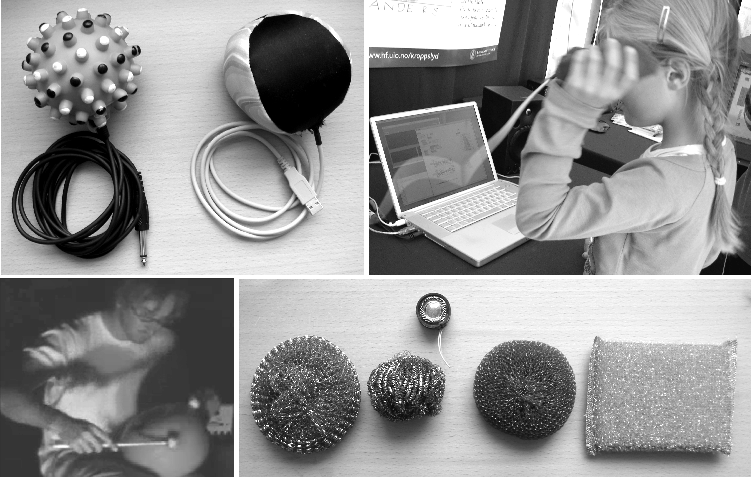
\includegraphics[width=\columnwidth]{figures/66-music-balls-crop.pdf}
	\caption{One acoustic and one electro-acoustic music ball (upper left). An electro-acoustic music ball in use at a research fair (upper right). Performance with a hybrid music ball (bottom right). A dynamic microphone element and various materials used inside of music balls (bottom right).}
	\label{fig:figures_music-balls_music-balls2}
\end{figure}

The first music balls I made focused on amplifying acoustic sounds. I would cut the ball and stuff them with various sound-producing objects, such as paper, peas, plastic, or steel wool. The challenge was to find materials that were both durable and nice-sounding. For example, newspaper sheets have a crisp sound when squeezed but contract quickly. Then plastic sponges work better since they expand quickly after being squeezed. The amplification of sound was done by placing microphones inside the balls. For some balls, I used contact microphones placed in the middle of the sounding material. Other times I used elements from broken dynamic microphones. Ripping out the microphone membrane and soldering on a new cable is an easy way of reusing the valuable parts. My favorite music balls are the ones that use dynamic microphone elements wrapped in steel wool. They produce clear and crisp sounds when amplified.

I have had much fun building and performing such music balls with students. Acoustic music balls can be assembled quickly in class, and they can be directly connected to a speaker or guitar amplifier. Many students have also explored using various sound effects in the chain, such as guitar pedals. Other times, we have connected the balls to a computer to extract sound features from the sound signal. Then the microphone signal can be used as a `sensor' to control digital sound synthesis. Combining these approaches is possible, effectively making the music ball into a hybrid device combining its audible sound with digital sound effects.

In most cases, I have focused on having only one microphone or one sensor per music ball. Sensor-based balls have often be built around an accelerometer or a pressure sensor placed inside a ball. Having only one sensor per ball makes them easy and cheap to produce. There are also fewer things to break. And, if a ball breaks, you have other balls available. Working with only one sensor per ball limits the interaction possibilities. An affordance-based interaction design also helps create more intuitive mappings. For example, an accelerometer-based music ball typically lends itself to creating sounds based on shaking the ball. On the other hand, a ball with a flex sensor inside affords to squeeze. At first, many students say they need more sensors to create interesting sonic results. However, when I tell them that they could also include time as a variable, they often develop creative sound interaction designs. There is a tendency to think about static mappings. Once you create a mapping, that is what you have. However, one of the potentials of electro-acoustic instruments is that you are not bound to the laws of nature. Creating mappings that change over time can be seen as a `gamification' strategy that may create excitement if done well. The trick is often to start with an ecologically meaningful mapping, which may evolve into something more creative. This is also a way of developing music-makers instead of sound-makers.


\section{Big Buoy} \label{sect:big-buoy}

After creating a range of small and simple music balls, I was challenged to make a big one for a research fair. This led to the creation of \emph{Big Buoy}, named so because we built it from a large ship buoy (Figure~\ref{fig:figures_giant-music-ball_09-Musikkball}). Here we ended up breaking with the initial `rule' of only using one or a few sensors per ball. One reason to include multiple sensors was that we developed Big Buoy as a multi-person instrument. Strangely enough, multi-person instruments are a rarity. Most musical instruments are built as a single-person device, although some---of which piano may be the most common---can be played by two. Contemporary multi-person instrument designs can often be found as museum installations rather than on stages. However, there are some exceptions, including the two-person instrument Tooka \citep{fels_tooka:_2002} and the multi-person reacTable \citep{jorda_reactable*_2005}.

Big Buoy was conceived of as a multi-person instrument. It was built so that it would not work well with less than four people playing concurrently. This called for more sensors, but we still tried to limit ourselves to only a few sensing modalities. Building on knowledge from the hybrid music balls, we placed strips of contact microphones and pressure sensors on the sides of the ball. This made it possible to pick up sound-producing actions with the microphones and use the sensors to control sound effects. Since the ball was hanging freely, we placed a 3D-accelerometer at the top to pick up motion patterns.

\begin{figure}[tbp]
	\centering
		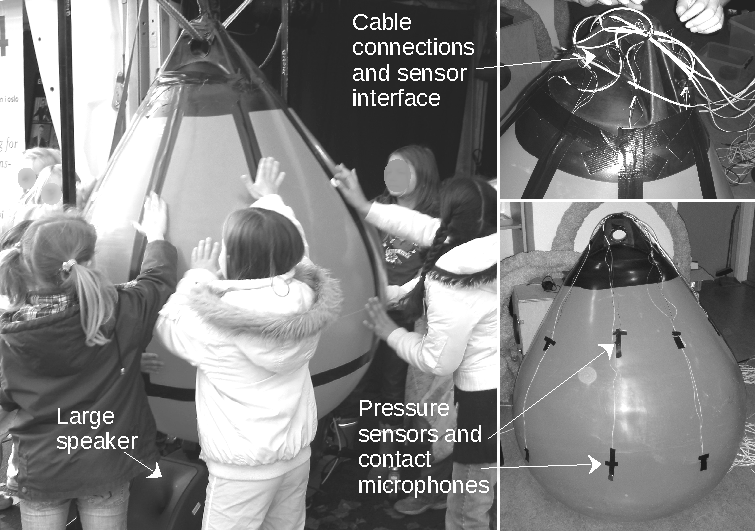
\includegraphics[width=1\columnwidth]{figures/67-big-buoy-crop.pdf}
	\caption{The Big Buoy is a multi-user instrument built with contact microphones and force sensing resistors.}
	\label{fig:figures_giant-music-ball_09-Musikkball}
\end{figure}

Before I started making music balls, I had not reflected much on the importance of local sound. However, when playing with multiple music balls, we quickly realized that it was necessary to separate the sound sources physically. The first attempts at connecting multiple music balls to a large PA system failed. The lack of local and directional sound was confusing both for performers and perceivers. We had therefore started to use small speakers close to each ball. We also experimented with placing speaker elements inside the balls, but this turned out to be tricky to realize given time constraints and limited engineering skills. For Big Buoy, we initially thought about embedding speakers inside of the ball. However, given the buoy's soft material, this turned out to be problematic from both a sound projection and interaction perspective. Instead, we placed a large PA speaker underneath the ball, which was large enough to produce low-frequency sounds matching the size of the ball.

We developed the initial mappings for Big Buoy based on previous experience playing music balls in various concert settings. However, when setting it up as an installation in Oslo's main shopping street, we quickly realized it was necessary to alter the mappings. For many coming by, our carefully developed action--sound mappings did not work well. The ball afforded rougher actions than we had anticipated. We, therefore, hastily adjusted the sound design to match the interaction mode. We also discovered that there was some time of day differences in the interaction patterns. More children were interacting with the ball in the mornings, while more adults came by in the afternoons. Hence, we also made two sets of mappings, with one being more `child-like.' In its first installation, thousands of people interacted with the ball. Many people commented positively about the unusual shape and size of the instrument.


\section{ADHD Ball} \label{sect:adhd}

An exciting possibility appeared when researchers at the Norwegian Institute of Public Health asked us to develop a music ball for clinical experiments on children with \emph{attention deficit hyperactivity disorder} (ADHD). They were running a large-scale, longitudinal study and wanted to engage the children while at the same time capturing information about their behavior. The idea was to make a music ball that would trigger different sound and light stimuli and collect data to study the childrens' response patterns. The ADHD ball was yet another exploration into the development of a musical instrument not meant to be an `instrument.' Rather, it was presented as a toy that the kids could play with when they came to their clinical testing at the hospital.

To allow for rough usage, we decided to develop a scaled-down version of Big Buoy. We used a similar buoy type, stripes of force-sensing resistors (FSRs) fastened to the surface and an accelerometer at the top (Figure~\ref{fig:figures_ADHD-ball}).
The buoy was padded with foam, and a heavy-duty party balloon was stretched around the buoy to serve as a protective outer skin. The ball was nice-looking and had a rubber-like tactile feel.

\begin{figure}[tbp]
	\centering
		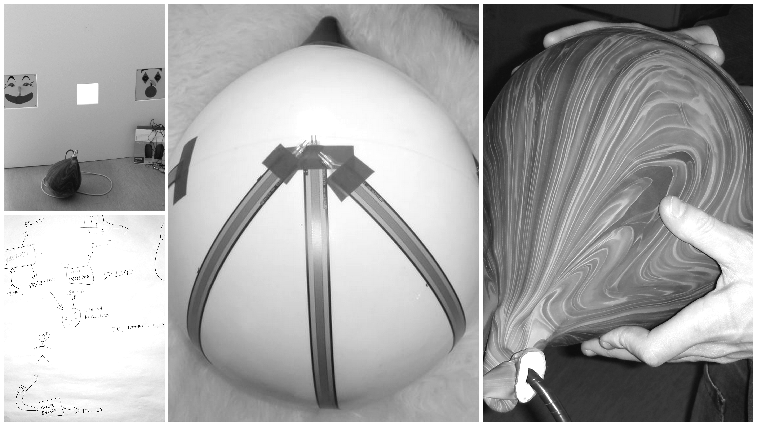
\includegraphics[width=1\columnwidth]{figures/68-adhd-ball-crop.pdf}
	\caption{Pictures from the design process (bottom left), sensor construction (middle), padding (right), and installation of the ADHD ball (upper left).}
	\label{fig:figures_ADHD-ball}
\end{figure}

The ball was popular with the kids and was in daily use for more than a year. Even though we had done our best to protect the electronics, we had to replace parts regularly. That is probably what to expect when you have continuous interaction over extended periods. Over time we also made slight adjustments to the action--sound mappings. Here we continued our experimentation with time-based mappings. This was done by changing sound material over time as if moving from one game level to another. If one would stop using the ball, the mappings would `reset' to their initial state, and the user would need to start playing again to reach the new levels. Such `gamification' helped to keep childrens' attention.


\section{Music Troll}

It is not ball-shaped, but the \emph{Music Troll} is yet another unconventional instrument designed with simplicity and playfulness in mind (Figure~\ref{fig:figures_music-troll_arj-troll}). The instrument was built as a `many-headed' device and named after the Scandinavian fairytale `troll' creature.
The idea was to create a collaborative interface based on different music balls. Like the construction of the small music balls, each head of the Music Troll was based on only one sensor type. In the end, we deviated slightly from the ball concept and, instead, made four heads of different shapes and sizes.

\begin{figure}[tbp]
	\centering
		\includegraphics[width=\columnwidth]{figures/69-music-troll-crop.pdf}
	\caption{Performing with the Music Troll in Oslo Concert Hall in October 2006.}
	\label{fig:figures_music-troll_arj-troll}
\end{figure}

The four heads covered different tonal and timbral ranges that fit well together. The first head was built with a dynamic microphone element surrounded by steel wool. The sound's envelope was used to control the speed and velocity of a voice sample played backward, creating a strange, voice-like sound. The second head was cone-shaped, with five `fingers' created by fastening strips to a plastic container with a dynamic microphone element inside. The sound from this microphone was amplified and compressed heavily to create a `squeaky' sound. The third dead was ball-shaped and contained a USB accelerometer controlling a percussive physical sound model. Finally, the fourth head was paddle-shaped with a long bend sensor inside that controlled a sweep filter on a synthetic sound.

Each of the heads was mounted to metal rods fixed to a custom-built wooden box. This box also contained all the necessary electronics, including a computer, sound card, amplifier, and speakers. There were four speakers, one on each side of the box, each playing sound from one head. That way, people could more easily hear their contribution when playing on the Music Troll collaboratively.

Similar to Big Buoy, the Music Troll was also built as a multi-person instrument. It was set up as an installation piece in public venues in the Oslo area several times. Also, this instrument received rough usage by thousands of people. As opposed to the open-ended interaction design of Big Buoy, the Music Troll had four separate heads with distinct musical sound designs. As such, it functioned primarily as a music-maker. People could control the sound on each head to some extent but within relatively narrow borders. This worked well to grab peoples' attention, but it did not encourage extensive musical explorations. I also did a few stage performances with the Music Troll (Figure~\ref{fig:figures_music-troll_arj-troll}). Then it was necessary to create different mappings, allowing for more nuanced control and the possibility of moving from head to head. However, performing alone was challenging. I had to move around the box to reach the heads, and the lack of co-performers led to a suboptimal experience.


\section{From prototype to prototype}

I have learned some lessons after designing and building many unconventional controllers and instruments over the years. First, I have learned that it can be rewarding to develop simple instruments with intuitive mappings. It is always tempting to add more sensors and features when developing instruments, but this may come at the cost of user engagement. Being forced to work with only a few sensing modalities leads to creative solutions. It also makes it possible to develop more devices. The music balls are not the most advanced instruments, but they are fun sound-makers. Some of them are also quite elaborate music-makers. One of my goals has been to show that making simple yet musically valuable technologies is possible. Just in the same way that one says that `the best camera is the one that you bring along,' we could say that the best instrument is the one you have at hand. Many of my students got an eye-opener when they understood that they could build an instrument themselves.

In my classes, students have built their own music balls from left-over materials: plastic, leather, wood, and fabric. The aim has been to show that it is possible to reuse materials. This is something we need to think more about in the future from an environmental perspective. The same is the case with repurposing technologies, such as reusing microphone parts. It is both cheaper and more sustainable. Reusing parts also led to more varied-looking technologies. We have also succeeded in creating `non-techy' instruments. Hiding the cables and electronics has been an essential part of why the devices have appealed to broader audiences.

Stability and durability are the two most significant drawbacks of all the devices presented in this chapter. Except for the ADHD ball, one could say that we have moved from prototype to prototype. \citet{NIME20_86} argue that there is a difference between an instrument prototype---a functioning but unfinished product---and a \emph{research product} that has the qualities of a finalized instrument. A research product is different from a commercial product in that it is made to produce knowledge. On the other hand, a commercial product results from an elaborate engineering process targeted at consumers. I think it makes sense to add yet another category to the list: \emph{research prototypes}. An instrument prototype may be made as a first step towards making a complete musical instrument. On the other hand, the primary function of a research prototype is to generate knowledge about the design process and how instruments can produce a particular type of musical experience. My experimentation with unconventional instrument designs was an eye-opener to understanding more about what an instrument can be. It also paved the way for `air instruments,' which we will look at in the next chapter.
